\documentclass[xetex,mathserif,serif]{beamer}
\usepackage{polyglossia}
\setdefaultlanguage[babelshorthands=true]{russian}
\usepackage{minted}
\usepackage{tabu}

\useoutertheme{infolines}

\usepackage{fontspec}
\setmainfont{FreeSans}
\newfontfamily{\russianfonttt}{FreeSans}

\usepackage{forest}
\usetikzlibrary{arrows}

\definecolor{links}{HTML}{2A1B81}
\hypersetup{colorlinks,linkcolor=,urlcolor=links}

\tabulinesep=0.7mm

\title{Стайлгайд, процесс компиляции}
\author[Юрий Литвинов]{Юрий Литвинов \newline \textcolor{gray}{\small\texttt{yurii.litvinov@gmail.com}}}

\date{17.09.2019}

\begin{document}
	
	\frame{\titlepage}
	
	\begin{frame}
		\frametitle{Стайлгайд}
		\begin{itemize}
			\item Программы пишутся для людей, а не для компьютера
			\item ``Школьник-стайл'' именования переменных (a, b, c1)
			\item Отступы!
			\item Пробелы!
			\item Правила именования
			\begin{itemize}
				\item Переменные со строчной, типы с заглавной
			\end{itemize}
			\item Компилироваться без предупреждений
			\item Не должно быть копипаста
			\item Один оператор на одной строке, и побольше фигурных скобок
		\end{itemize}
	\end{frame}

	\begin{frame}
		\frametitle{Стайлгайд}
		\begin{itemize}
			\item По возможности сужайте области видимости переменных
			\item Используйте самые узкие типы из подходящих (например, bool)
			\item Переменные --- это плохо, константы --- хорошо
			\item Глобальные переменные --- это очень, очень плохо
			\item goto --- это вообще ужасно
			\item Одна сущность должна играть одну роль в программе
			\begin{itemize}
				\item Одна функция должна делать одно дело
				\item Одна переменная должна означать что-то одно
			\end{itemize}
			\item Бинарные операторы и ключевые слова выделяются пробелами
			\item \url{http://se.math.spbu.ru/SE/Members/ylitvinov/styleguide}
		\end{itemize}
	\end{frame}

	\begin{frame}
		\frametitle{Процесс компиляции С++}
		\begin{center}
			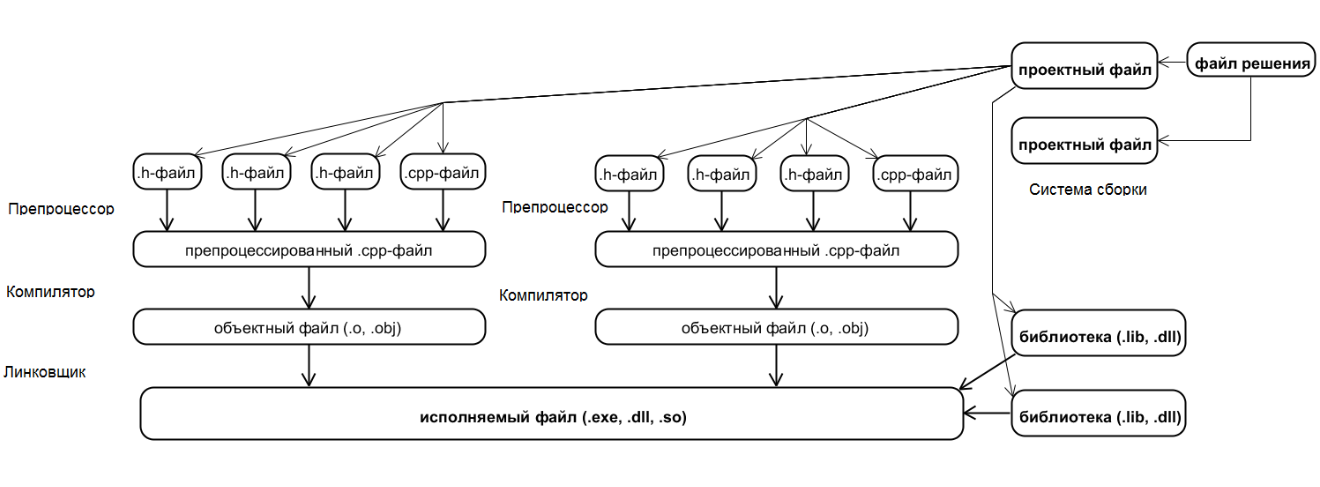
\includegraphics[width=0.95\textwidth]{compilation.png}
		\end{center}
	\end{frame}

	\begin{frame}
		\frametitle{Указатели и куча}
		\begin{center}
			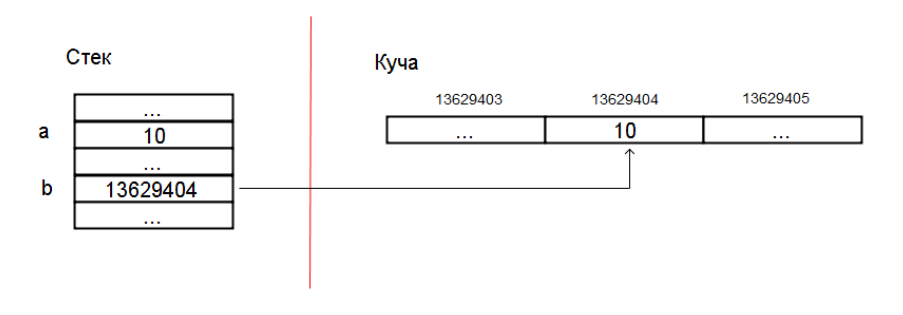
\includegraphics[width=0.8\textwidth]{pointers.png}
		\end{center}
	\end{frame}

\end{document}

